\documentclass[../TDT5.tex]{subfiles}%

\begin{document}
\section{Pompe à chaleur domestique}
\enonce{%
	On veut maintenir la température d'une maison à $T_1 =
		\SI{20}{\degreeCelsius}$ alors que la température extérieure est égale à $T_2
		= \SI{5}{\degreeCelsius}$, en utilisant une pompe à chaleur. L'isolation
	thermique de la maison est telle qu'il faut lui fournir un transfert thermique
	égal à \SI{200}{kJ} par heure pour cet effet.
}%
\QR{%
	Rappeler le schéma de principe d'une pompe à chaleur ditherme et le sens réel
	des échanges d'énergie du fluide caloporteur.
}{%
	~
	\smallbreak
	\vspace{-15pt}
	\noindent
	\begin{minipage}[c]{.65\linewidth}
		Une pompe à chaleur reçoit un transfert thermique de la source froide ($Q_F =
			Q_2 > 0$) et cède un transfert thermique à la source chaude ($Q_C = Q_1 < 0$).
		Cela nécessite de lui apporter un travail ($W > 0$).
	\end{minipage}
	\hfill
	\begin{minipage}[c]{.30\linewidth}
		\vspace{0pt}
		\begin{center}
			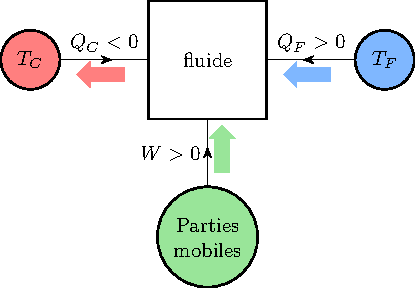
\includegraphics[width=\linewidth]{refrig_dth}
		\end{center}
	\end{minipage}
}%
\QR{%
	Quel doit être le cycle thermodynamique suivi par le fluide pour que
	l'efficacité de la pompe à chaleur soit maximale~?
}{%
	Le cycle d'efficacité maximale est le \textbf{cycle de \textsc{Carnot}},
	composé de deux isothermes aux températures des sources et de deux
	adiabatiques réversibles.
}%
\QR{%
	Définir et calculer l'efficacité théorique maximale de la pompe dans ces
	conditions. Montrer qu'elle ne dépend que de la différence de température
	entre l'intérieur et l'extérieur. Quel est le sens physique de l'efficacité~?
}{%
	\begin{DispWithArrows*}[groups]
		e\sup{PAC} &=
		\frac{-Q_C}{W} =
		\frac{Q_C}{Q_C+Q_F}
		\\\Lra
		e\sup{PAC} &=  \frac{1}{1+\frac{Q_F}{Q_C}}
		\Arrow{$\frac{Q_F}{T_F} \leq -\frac{Q_C}{T_C}$\\Or,
			$Q_C < 0$\\$1+\frac{Q_F}{Q_C} \geq 1 - \frac{T_F}{T_C}$}
		\\\Lra
		e\sup{PAC} &\leq \frac{1}{1 - \frac{T_C}{T_F}}
		\\\Lra
		e\sup{PAC} &\leq \boxed{\frac{T_C}{T_C-T_F} = e_C\sup{PAC}}
		\\\Ra
		\Aboxed{e_C\sup{PAC} &= \frac{T_1}{T_1-T_2}}
		\Ra
		\xul{e_C\sup{PAC} = \num{20}}
	\end{DispWithArrows*}
	L'efficacité quantifie la performance énergétique de la PAC~: pour
	\SI{1}{J} d'énergie électrique fournie au moteur, on récupère $e$ joules
	de transfert thermique cédé à la source chaude.
}%
\QR{%
	En déduire la puissance électrique minimale consommée par la pompe à
	chaleur.
}{%
	Par définition, s'il faut fournir un travail $W$ à la PAC pendant une durée
	$\Delta{t}$, alors la puissance électrique minimale qu'elle consomme vaut
	$\Pc\ind{élec} = W/\Delta{t}$. C'est un minimum, car le rendement du moteur
	électrique qui permet l'écoulement de fluide dans la PAC n'est sûrement pas de
	1. L'énoncé donne par ailleur la puissance thermique $\Pc\ind{th} =
		Q_C/\Delta{t} = \SI{0.55}{W}$ qu'il faut apporter à la maison pour
	maintenir sa témpérature constante. En utilisant la définition de
	l'efficatié, on en déduit
	\[
		e = \frac{\Pc\ind{th}\Delta{t}}{\Pc\ind{élec}\Delta{t}}
		\Lra
		\boxed{\Pc\ind{élec} = \frac{\Pc\ind{th}}{e}}
		\Ra
		\xul{\Pc\ind{élec} = \SI{2.8}{kW}}
	\]
}%
\QR{%
	En supposant la température intérieure imposée, pour quelle température
	extérieure l'efficacité est-elle maximale~?
}{%
	L'efficacité de la PAC augmente lorsque la différence de témpérature entre les
	soures décroît, elle est optimale lorsque les deux sources ont la même
	température… mais alors il n'y a plus besoin de chauffer~! En tout état de
	cause, il vaut mieux utiliser une PAC avec un chauffage au sol plutôt que par
	radiateurs car l'eau de chauffage y est moins chaude
	($\SI{35}{\degreeCelsius}$ contre $\SI{60}{\degreeCelsius}$).
}%

\end{document}
